\section{Caracterizando rutas}

\subsection{Estimación del RTT}
A partir de la tool implementada, que permite realizar un \textbf{traceroute}, se pueden obtener los RTT entre cada salto de hops para una ruta a una IP determinada. De esta manera, se plantea en primer lugar 4 universidades diferentes, que serán utilizadas para poder llevar a cabo el análisis necesario utilizando la herramienta.

\begin{itemize}
 \item {\bf Universidad Humboldt de Berlín}

	{\bf Distancia}: 11910 km

	{\bf IP}: 141.20.5.188 (\url{www.hu-berlin.de}{})

 \item {\bf Universidad de Moscú}

	{\bf Distancia}: 13484 km

	{\bf IP}: 188.44.33.1 (\url{www.msu.ru}{})

 \item {\bf Universidad de Boston}

	{\bf Distancia}: 8680 km

	{\bf IP}: 54.230.225.44 (\url{www.bu.edu}{})

 \item {\bf Universidad de Tokio}

	{\bf Distancia}: 18360 km

	{\bf IP}: 210.152.135.178 (\url{www.u-tokyo.ac.jp}{})

\end{itemize}

Las distancias descriptas corresponden a la distancia lineal que hay entre la universidad y un punto en común en Buenos Aires. La misma se obtuvo utilizando una opción dada por Google Maps \footnote{\url{maps.google.com}{}}. Ese dato se podrá utilizar para poder obtener el RTT teórico y aproximado de un paquete para cada una de las universidad a analizar.

Asumiendo que los enlaces son siempre de fibra óptica, y que el velocidad de propagación de las señales es de $2 \times 10^{5}$ km/s podemos estimar el RTT de la siguiente manera:

\begin{itemize}
 \item Universidad Humboldt de Berlín:
\begin{equation}
 	RTT = 2 \times T_{prop} = 2 \times (Dist / V_{prop}) = 2 \times (11910 \text{ km} / 2\times10^5 \text{ km/s}) = 119.1  \text{ ms}
\end{equation}

 \item Universidad de Moscú:
 \begin{equation}
 	RTT = 2 \times T_{prop} = 2 \times (Dist / V_{prop}) = 2 \times (13484 \text{ km} / 2\times10^5 \text{ km/s}) = 134.84 \text{ ms}
 \end{equation}

 \item Universidad de Boston:
 \begin{equation}
 	RTT = 2 \times T_{prop} = 2 \times (Dist / V_{prop}) = 2 \times (8680 \text{ km} / 2\times10^5 \text{ km/s}) = 86.8 \text{ ms}
 \end{equation}

 \item Universidad de Tokio:
 \begin{equation}
 	RTT = 2 \times T_{prop} = 2 \times (Dist / V_{prop}) = 2 \times (18360  \text{ km} / 2\times10^5 \text{ km/s}) = 183.6 \text{ ms}
 \end{equation}

\end{itemize}

El valor obtenido representa un cota inferior muy burda del tiempo de comunicación entre Buenos Aires y las universidades seleccionadas. Esto se debe a que no contempla los obstáculos que se presentan desde que un paquete sale del hop inicial y llega a destino. Hay ciertas situaciones que fomentan un aumento importante del tiempo de RTT del mensaje. Se presenta a continuación, las diferencias entre el RTT teórico y el obtenido utilizando una herramienta brindada por el sistema operativo \footnote{\url{http://ping.eu}{}}.

\centerline{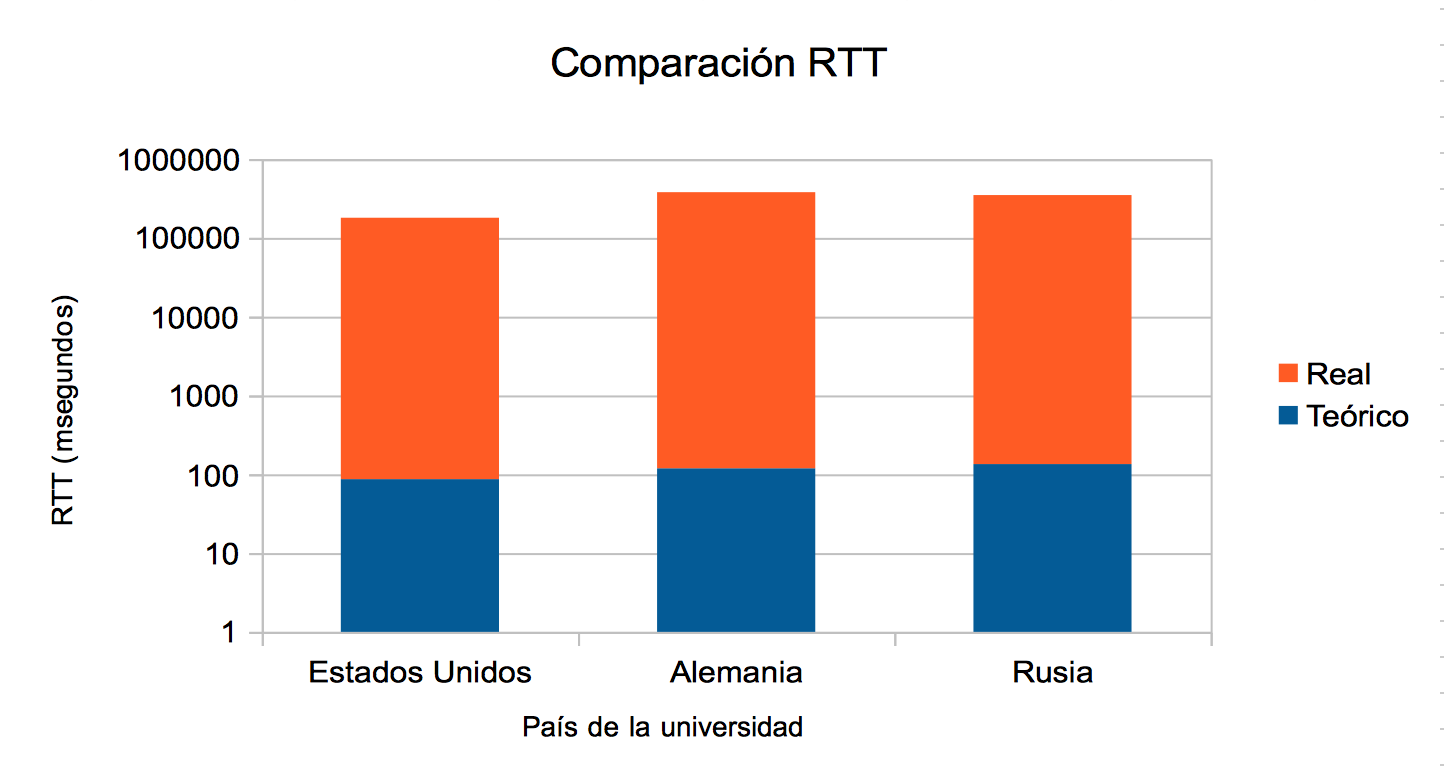
\includegraphics[width=0.8\textwidth]{imagenes/1ra_parte/1Parte-comparacionRTT}}

Se muestran los resultado utilizando escala logarítmica para poder observarlos de manera clara. A lo largo del trabajo práctico se podrán ir observando las situaciones que hacen a que el RTT teórico sea tanto menor que el real.

Por otro lado, se decide comparar la herramienta desarrollada utilizando Scapy, contra el traceroute brindado por el sistema operativo. Ambos traceroutes envían una cierta cantidad de paquetes a cada host intermedio que se tiene para llegar al de destino, y miden el tiempo obtenido. Luego, se realiza un promedio del mismo. A continuación, se presentan los RTT obtenidos para cada host intermedio utilizando ambas herramientas. 

\centerline{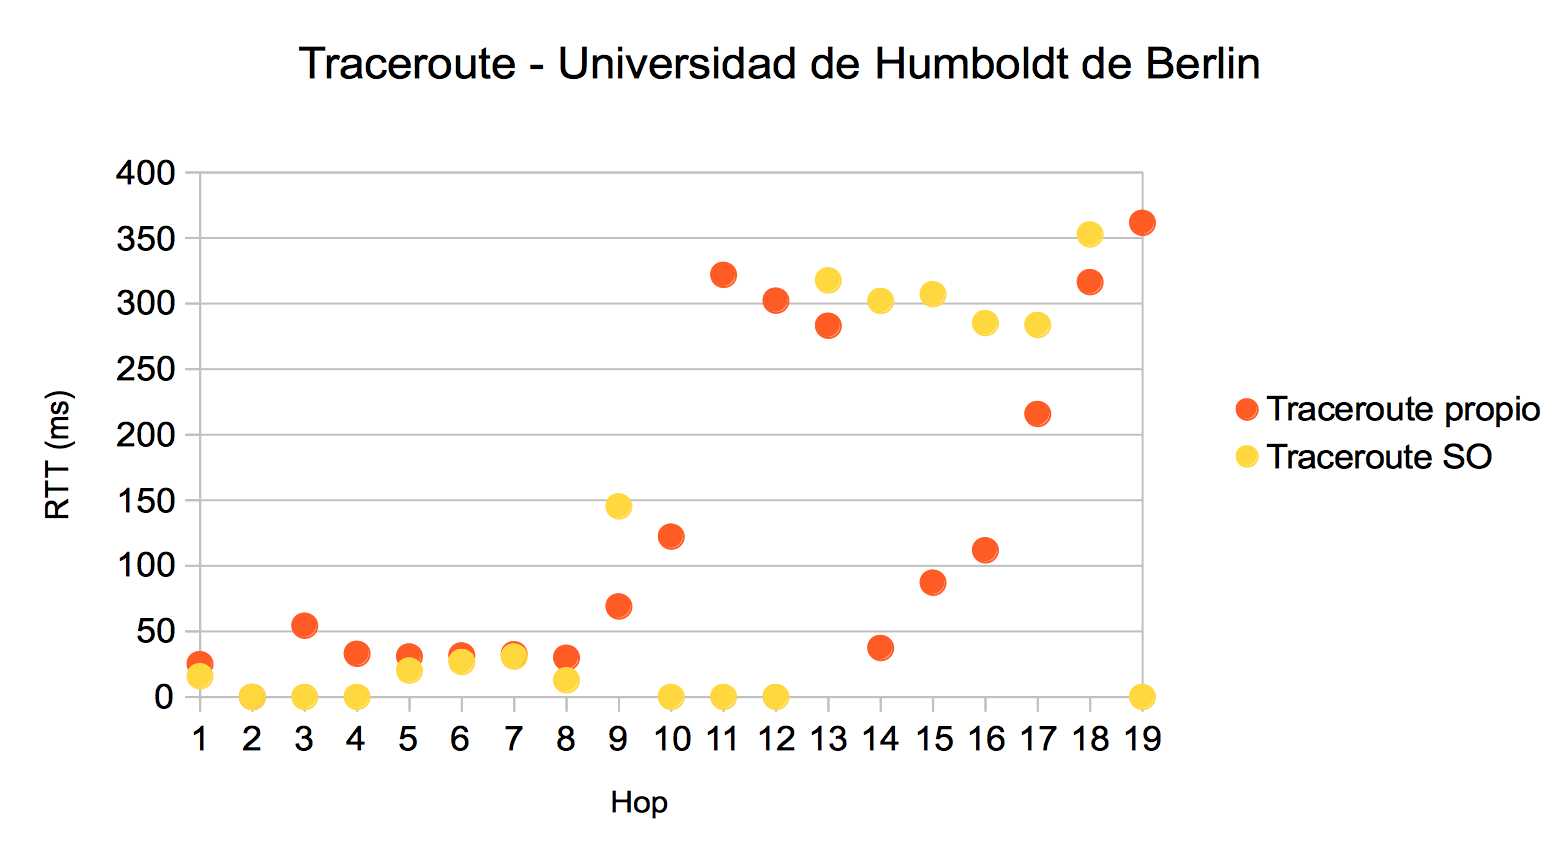
\includegraphics[width=1\textwidth]{imagenes/1ra_parte/Alemania_1ergrafico.png}}

\centerline{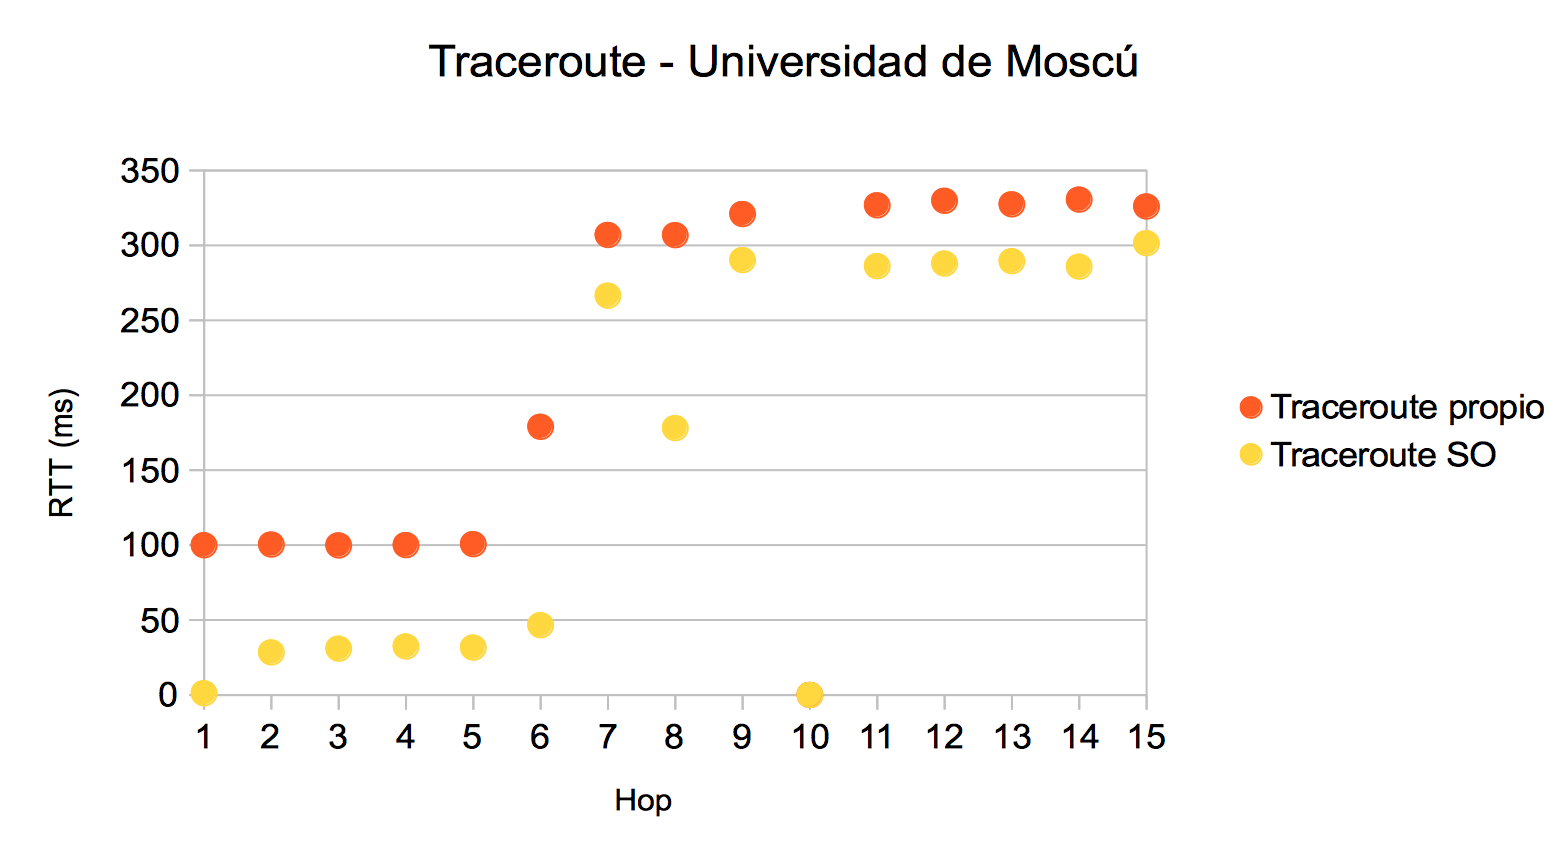
\includegraphics[width=1\textwidth]{imagenes/1ra_parte/Rusia_1ergrafico.png}}

\centerline{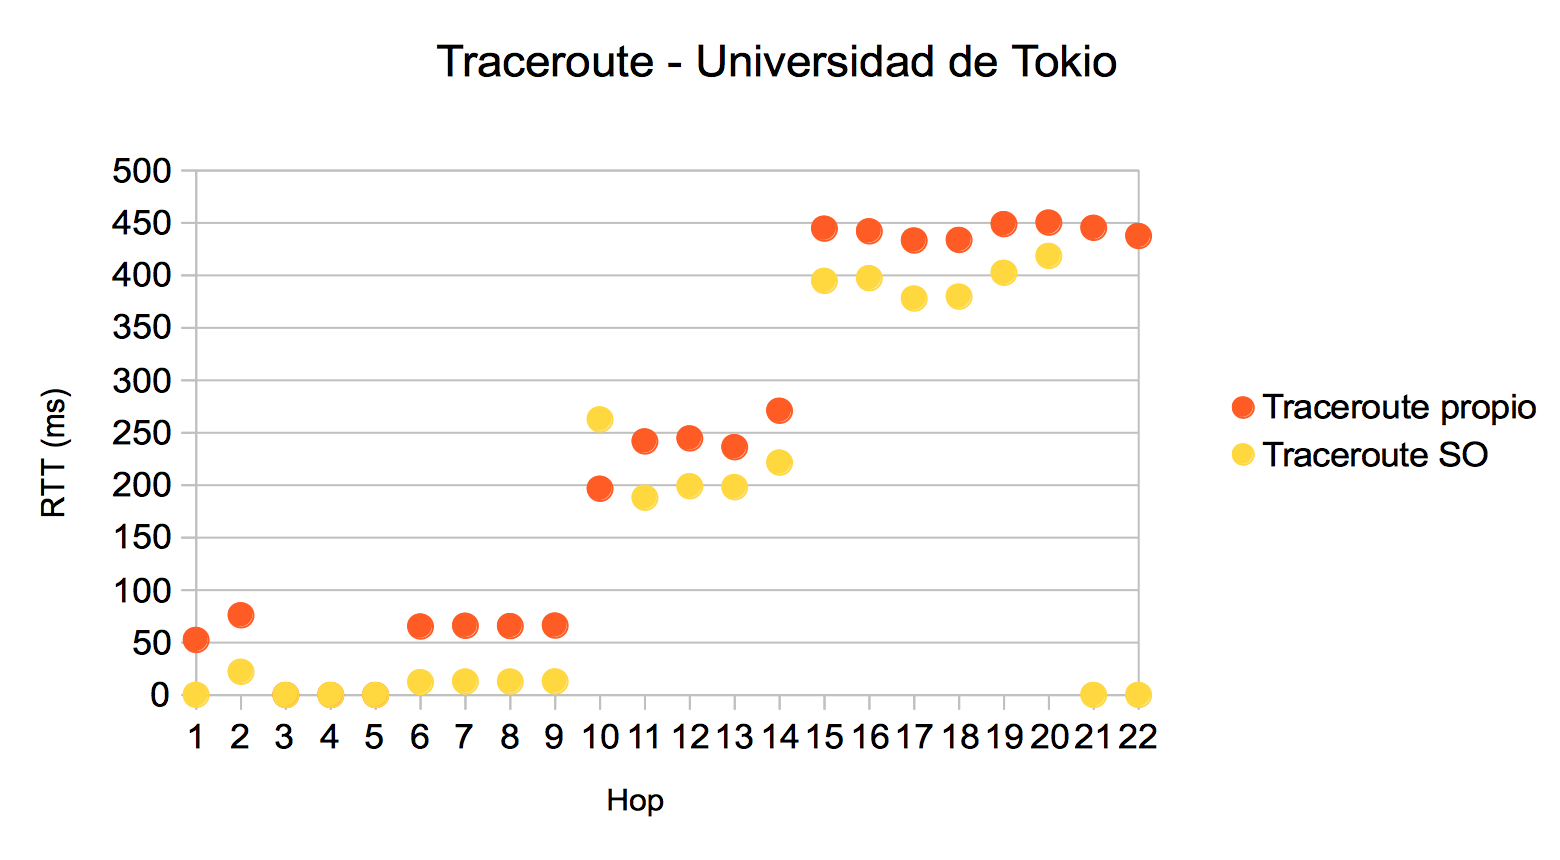
\includegraphics[width=1\textwidth]{imagenes/1ra_parte/Japon_1ergrafico.png}}

\centerline{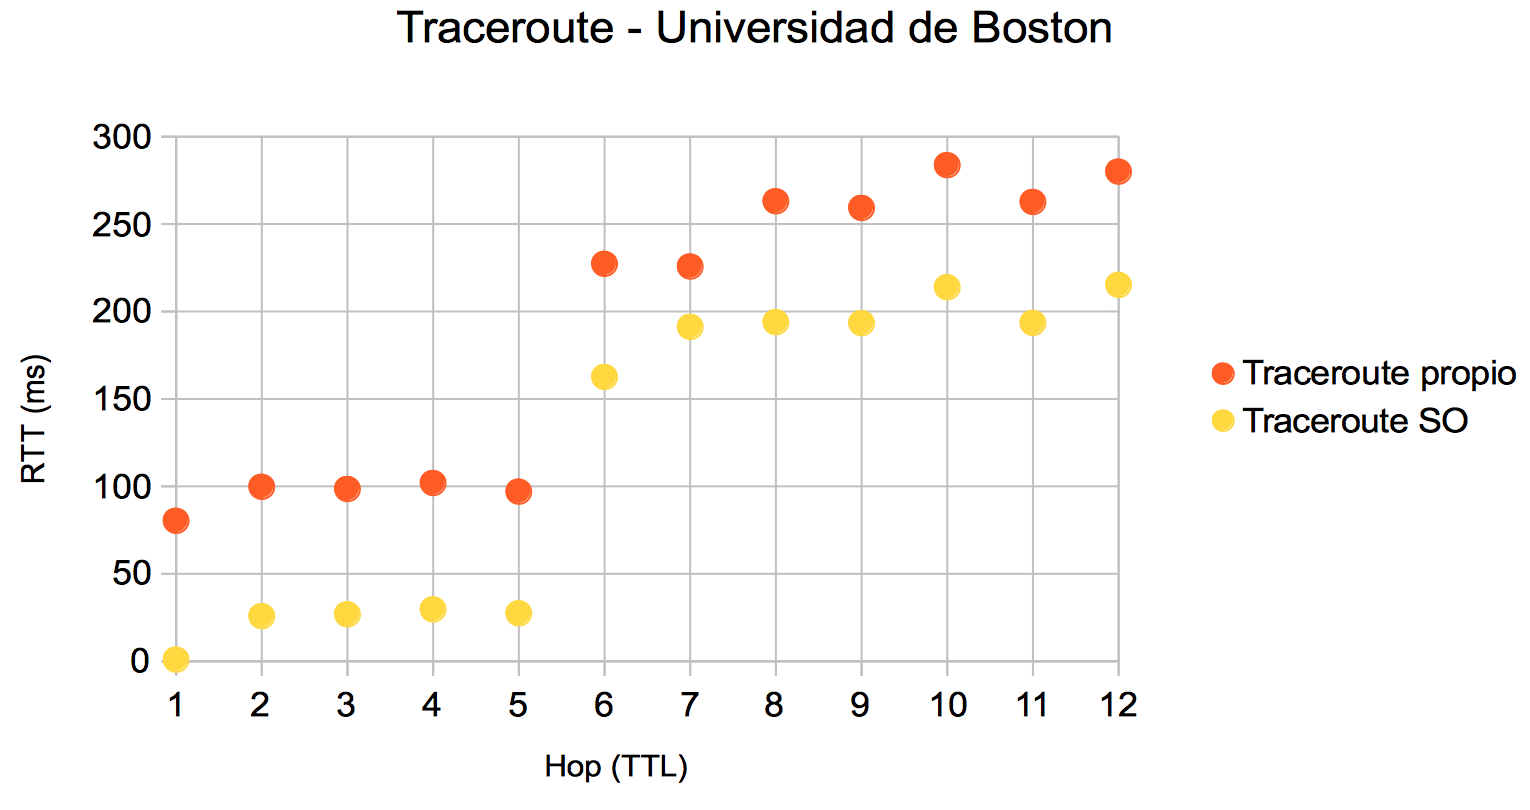
\includegraphics[width=1\textwidth]{imagenes/1ra_parte/EEUU_1ergrafico.png}}

Los gráficos presentados permitieron obtener diversas conclusiones con respecto al comportamiento de los paquetes en las distintas redes. Estos comportamientos se ven reflados en los tiempos de RTT que presenta cada paquete para cada TTL. A continuación enumeranemos los escenarios que se pudieron encontrar y que generan inconsistencias en las mediciones:
\begin{itemize}
\item Existe más de un ruta posible para un cierto número de TTL para un mismo host de destino. En el caso de la herramienta de traceroute desarrollada por nosotros, no se distingue por host sino por número de TTL. Es decir, el promedio de RTT obtenido a partir de mil paquetes enviados con una misma IP destino y TTL, se realizará sin distinguir si la dirección IP correspondiente a la respuesta es siempre el mismo. Existe una amplia red de routers intermedios que se pueden utilizar para llegar a un mismo destino. En el caso del traceroute brindado por el sistema operativo, se realiza el promedio sobre únicamente tres paquetes diferentes, dándose mayormente que tengan la misma dirección IP. 

\item Hay host intermedios a un destino final que pueden no responder a un ping enviado. Esto puede deberse a que los mismos no estan configurados para responder a este tipo de pedido o que esten congestionados de manera tal de no llegar a responder a tiempo. En el primer caso, no importa la herramienta que se utilice, el resultado siempre será el mismo. Pero, para el segundo escenario planteado, la herramienta brindada por el sistema operativo no intenta resolver la problemática. Sin embargo, en la desarrollada para este trabajo práctico, se basa en el envío de mil paquetes a un mismo TTL, es decir, que el congestionamiento del host podrá liberarse para alguno de los pedidos y la respuesta llegará antes del time out, pudiendose así obtener un RTT estimado. El RTT promedio obtenido del envío de los mil paquetes descarta aquellos que tuvieron time-out para así no disminuir el valor final.

\item Un caso que no es contemplado en ninguno de las dos herramientas utilizadas, es que la ruta que siga un paquete, pasando por una determinada cantidad de hops, sea siempre la misma. Para el cálculo de los RTT no se contempla que una ruta pueda tomar más tiempo que otra, ya que no se tiene forma de saber cual es el camino exacto que realiza un mensaje para llegar a un determinado host. En el caso de la herramienta desarrollada se simula el paso del paquete por distintos host hasta llegar el de la universidad deseada, pero con respecto a los RTT de los hop intermedios, se los trata sin distinguir la ruta que realizan. 


\end{itemize}



Uno de los motivos que afecta a los tiempos en los que un paquete tarda en llegar a un host y luego retornar, es el del congestionamiento que puede existir en la red. El mismo surge a partir de un alto número de paquetes existentes en la misma, debido a un gran número de personas que intentan conectarse a un mismo lugar. Para poder observar este comportamiento, es decir, los fluctuantes valores de RTT para cada hop intermedio, se realizó el siguiente experimento, el cual consiste en analizar el tráfico de la red en distintas horas del día. Para ello se ejecutó el traceroute desarrollado en tres horarios diferentes. Se obtienen los siguientes gráficos:

%\centerline{\includegraphics[width=0.8\textwidth]{.imagenes/traceroute_empirico_alemania.png}}

%\centerline{\includegraphics[width=0.8\textwidth]{.imagenes/traceroute_empirico_moscu.png}}

%\centerline{\includegraphics[width=0.8\textwidth]{.imagenes/traceroute_empirico_eeuu.png}}

%\centerline{\includegraphics[width=0.8\textwidth]{.imagenes/traceroute_empirico_japon.png}}

Conclusiones de eso..

Luego, se agrega a la herramienta desarrollada por nosotros, un agregado para que se calcule el valor standard (ZRTT) de cada salto con respecto a la ruta global. El cálculo a realizarse es el siguiente:

 \begin{equation}
 	ZRTT_i = \frac{RTT_i - \overline{RTT}}{SRTT} 
 \end{equation}

 Siendo RTT$_{i}$ el RTT medido para el salto entre host número i, $\overline{RTT}$ el promedio para los RTT de todos los saltos realizados y por último el SRTT representa el desvío standard de los RTTs de la ruta, y se calcula de la siguiente manera:

\begin{equation}
 	SRTT = \sqrt{\frac{1}{n} \sum_{i=1}^{n} (RTT_i - \overline{RTT})^2}
 \end{equation}

El ZRTT nos permite definir de forma rápida y exacta cuánto se aleja un RTT de un salto específico respecto al promedio. Luego se podrán realizar diversos análisis y conclusiones utilizando los valores obtenidos en los siguientes gráficos. Estos últimos representan el ZRTT calculado para una medición hecha con mil paquetes para cada TTL con destino cada una de las universidades definidas previamente. 

%\centerline{\includegraphics[width=0.8\textwidth]{.imagenes/traceroute_empirico_alemania.png}}

%\centerline{\includegraphics[width=0.8\textwidth]{.imagenes/traceroute_empirico_moscu.png}}

%\centerline{\includegraphics[width=0.8\textwidth]{.imagenes/traceroute_empirico_eeuu.png}}

%\centerline{\includegraphics[width=0.8\textwidth]{.imagenes/traceroute_empirico_japon.png}}

